\documentclass{article}

\usepackage{amsmath, amssymb, graphicx}
\usepackage{tikz}

\title{Regular Path Queries in Graph Databases}
\date{\today}
\author{Lewis Dyer}

\begin{document}
\maketitle

\begin{itemize}
    \item Formally define Regular Path Queries, and give an example or two.
    \item Formally introduce the main semantics of regular path queries, defining the main algorithmic questions in play.
    \item Give some results so far.
\end{itemize}

\section{Preliminaries}
\label{sec:prelims}

As a model for graph databases, we consider directed edge-labelled graphs. Given an alphabet $\Sigma$, a graph $G = (V,E)$ consists of a set of vertices $V$, along with a set of edges $E \subseteq (V \times \Sigma \times V)$, with $(u, l, v)$ denoting at edge from vertex $u$ to vertex $b$ with label $l$. Note that this model requires that every edge is labeled, and that we may omit the label if this label is irrelevant or clear from context. We further note that loops and multiple edges are permitted in this model.

Given two vertices $u$ and $v$, a path $p$ is defined by a sequence of edges of the form $(v_0, l_1, v_1), (v_1, l_2, v_2), \dots, (v_{n-1}, l_n, v_n)$ where $u = v_0$ and $v = v_1$, and we say this path has length $n$. We denote $\mathcal{P}_(G, u ,v)$ as the set of all such paths in $G$ between $u$ and $v$, occasionally omitting the subscript where this is clear from context.  We say a path is $\emph{simple}$ if any two vertices $v_i, v_j$ in $p$ are pairwise distinct.

\section{Introducing regular path queries}
\label{sec:intro_rpqs}

Given a path $p$ in a graph $G$ and vertices $u$ and $v$, we consider the word $w_p$ formed in $\Sigma^*$ by concatenating each edge label in $p$. More formally, the function $w: \mathcal{P}_{(G,u,v)} \rightarrow \Sigma^*$ with $w \left((v_0, l_1, v_1), (v_1, l_2, v_2), \dots, (v_{n-1}, l_n, v_n) \right) = l_1 l_2 \dots l_n$ produces the unique word associated with a given path $p$. Regular path queries (also denoted as RPQs) consist of a regular expression $r$ along with a set of \emph{semantics} for that RPQ, though we frequently refer to an RPQ solely by the regular expression where the semantics being used are clear from context. Evaluating an RPQ over a graph $G$ between vertices $u$ and $v$ consists of two steps: first, we consider paths $p \in \mathcal{P}_{(G,u,v)}$ such that $w(p)$ is accepted by $r$, and we denote these paths as the set of \emph{candidate paths} of the RPQ. Then, we determine which of these candidate paths to output depending on the semantics being used. Three typical sets of semantics are:

\begin{itemize}
    \item \textbf{Arbitrary semantics}, where all candidate paths are returned.
    \item \textbf{Shortest path semantics}, where all candidate paths of minimum length are returned.
    \item \textbf{Simple path semantics}, where all simple candidate paths are returned.
\end{itemize}

\begin{figure}
    \centering
    \label{fig:arbitrary_infinite}
    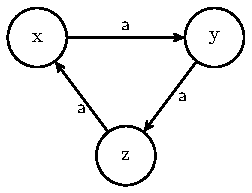
\includegraphics{figures/arbitrary_infinite.pdf}
    \caption{A directed cyclic graph on $3$ vertices, where every edge has label $a$.}
\end{figure}

Each of these sets of semantics presents different challenges. When using arbitrary semantics, care must be taken to avoid paths of infinite length, which can occur in cyclic directed graphs. For example, evaluating $a^*$ over the graph in Figure \ref{fig:arbitrary_infinite} from vertex $x$ to vertex $y$ using arbitrary semantics will result in an infinite set of paths with words given by the set $\{a^{3k+1} | k \in \mathbb{N}\}$.

Shortest path semantics avoid this problem, but can be counter-intuitive even for common queries. For example, when counting the number of paths between two vertices $x$ and $y$ that are accepted by some regular expression $r$, adding an additional path between $x$ and $y$ can actually reduce the overall count, if this newly added path is accepted by $r$ and is shorter than any other paths.

Simple paths avoid this lack of intuition while also avoiding paths of infinite length, and correspond to many natural constraints on paths in common queries. For example, in a transport network where vertices correspond to locations and edges correspond to different forms of travel between locations, finding simple paths between two locations means that visiting the same location more than once is not permitted.


\section{Complexity of evaluating RPQs}
\label{sec:complexity}

To begin, we first formalise the set of evaluation problems on RPQs we are considering. We define the decision RPQ evaluation problem with arbitrary path semantics as follows:

\fbox{\parbox{\textwidth}{
\textsc{Path}

\textbf{Input:} A graph $G$ with a starting vertex $s$ and an ending vertex $e$, and a regular expression $r$.\\

\textbf{Output:} \texttt{true} if there exists a path $p$ in $G$ matching $s$ and $r$ such that $w(p)$ is accepted by $r$, and \texttt{false} otherwise.
}} \\

Note that this defines the decision problem for RPQ evaluation under arbitrary path semantics. Analogous variants of this decision problem exist for the other forms of semantics introduced in Section \ref{sec:intro_rpqs}, which we shall denote as \textsc{ShortPath} and \text{SimPath} for shortest path and simple path semantics respectively. Similarly, we may also define enumeration variants of these problems, where all such paths from $s$ to $r$ whose words are accepted by $r$ should be returned. We denote these problems as \textsc{EnumPaths}, \textsc{EnumShortPaths} and \textsc{EnumSimPaths}.



\section{Characterising RPQs for simple path semantics}
\label{sec:simple_characterisation}

As discussed in Section \ref{sec:complexity}, \textsc{SimPath} and \textsc{EnumSimPaths} are in general intractable over all possible regular expressions, with \textsc{SimPath} being NP-complete with the regular expression $(aa)^*$ and \textsc{EnumSimPaths} being \#P-complete with the regular expression $a^*$. A natural further question is whether a particular class of regular expressions allows for tractable decision and enumeration, and moreover whether this class is sufficiently powerful to handle regular path queries that are used in practice.


\end{document}

